\subsection{Radiating Sources in TEM Cells}

\subsubsection{Arbitrary source}

Suppose a current source $\mathbf{J}_1$ excites a waveguide (as is the case with the dipoles in the TEM cell). Normally, such a current source requires external fields to drive it, but for they are neglect for now. Only $\mathbf{E}$ and $\mathbf{H}$ are considered, which are the fields radiated by $\mathbf{J}_1$. $\mathbf{E}$ and $\mathbf{H}$ are solved according to $\nabla \times \mathbf{E}=-j\omega\mu_0\mathbf{H}$ and $\nabla\times\mathbf{H}=j\omega\epsilon_0\mathbf{E}+\mathbf{J}$ \cite[p. 360]{Collin_2015}. Additionally, $\mathbf{e}_n^\pm$ and $\mathbf{h}_n^\pm$ are the resulting waveguide fields, with the signs indicating the direction of propagation. Take \autoref{eqn:lorentz_rec_theorem_int} and set $\mathbf{J}_2=\mathbf{M}_1=\mathbf{M}_2=0$. Now, only the current source $\mathbf{J}_1$ remains, and the \autoref{eqn:J1_propagating_waves} emerges. % Explain how certain surfaces do not to have be integrated, therefore rendering this equation very useful. Also, the expansion coefficients can be determined. Maybe do this calculation with a rectangular waveguide.

\begin{equation}
	\oiint _S (\mathbf{e}_n^\pm\times \mathbf{H}-\mathbf{E}\times \mathbf{h}_n^\pm)\cdot\mathrm{d}\mathbf{s'}=\iiint \mathbf{J_1}\cdot\mathbf{e}_n^\pm\mathrm{d}v'
	\label{eqn:J1_propagating_waves}
\end{equation}

\begin{figure}[htbp]
	\centering
	\includegraphics[width=0.7\linewidth]{content/img/reciprocity_tem_cell}
	\caption{TEM cell with an arbitrary current source $\mathbf{J}_1$ along the curve $\boldsymbol{\tau}$. $\mathbf{E}$ and $\mathbf{H}$ are the field intensities induced by the current. $\mathbf{e}^+_n$ and $\mathbf{e}^-_n$ are outgoing fields towards both output ports of the TEM cell of arbitrary form. $\mathbf{S}$ indicates the surface, and $V$ the volume of the domain in question.}
	\label{fig:reciprocitytemcell}
\end{figure}

\todo[inline]{TODO: Maybe add H fields in figure?}

%In case of the TEM cell, it is desirable that only the TEM mode is propagating, and that the source is represented by a dipole. 

The fields $\mathbf{E}$ and $\mathbf{H}$ radiated by $\mathbf{J}_1$ equal a combination of normals modes. Using the expansions \cref{eqn:a_modal_superposition1,eqn:a_modal_superposition2}, \cref{eqn:b_modal_superposition1,eqn:b_modal_superposition2} lead to

\begin{align}
	\oiint _S (\mathbf{e}_n^+\times \mathbf{H}-&\mathbf{E}\times \mathbf{h}_n^+)\cdot\mathrm{d}\mathbf{s'}=\nonumber\\ \nonumber
	&=\oiint _S (\mathbf{e}_n^+\times \sum_m a_m\mathbf{h}_m^+-\sum_m a_m\mathbf{e}_m^+\times \mathbf{h}_n^+)\cdot\mathrm{d}\mathbf{s'}\\
	&=\sum_m a_m \oiint _S (\mathbf{e}_n^+\times \mathbf{h}_m^+-\mathbf{e}_m^+\times \mathbf{h}_n^+)\cdot\mathrm{d}\mathbf{s'}.
\end{align}

Due to the orthogonal property of \autoref{eqn:norm_power} and the normalization in \autoref{eqn:unit_power}, the coefficients of each mode can be evaluated separately through

\begin{align}
	\oiint _S (\mathbf{e_n^+}\times \mathbf{H}&-\mathbf{E}\times \mathbf{h}_n^+)\cdot\mathrm{d}\mathbf{s'}=\nonumber\\
	&=a_n \oiint _S (\mathbf{e}_n^+\times \mathbf{h}_n^+-\mathbf{e}_n^+\times \mathbf{h}_n^+)\cdot\mathrm{d}\mathbf{s'}=-2a_n.
\end{align}

The coefficient $b_n$ of the fields $\mathbf{e}_n^-$ and $\mathbf{h}_n^-$ are evaluated in the same manner.

In this equation, the wave amplitudes $a_n$ and $b_n$ are given through the surface integral in the Lorentz Reciprocity theorem, with $a_n$ being the wave going to the left side, and $b_n$ to the other. 

One pair of coefficients $a_\mathrm{TEM}$, $b_\mathrm{TEM}$ suffice when investigating the propagation of the TEM mode, only. The fields $\mathbf{e}_\mathrm{TEM}$ and $\mathbf{h}_\mathrm{TEM}$ of the TEM-mode are known \todo{Some plot or table for explanation, plus citation}. Combining them with \autoref{eqn:unit_power} leads to \cite{4091811}

\begin{subequations}
	\begin{equation}
		P_{\mathrm{out1}}=\iint_S \langle \mathbf{S} \rangle \cdot \mathrm{d}\mathbf{s'}= \iint_S \frac{1}{2} \, \Re \{ \left(a\cdot \mathbf{e}_\mathrm{TEM}^\pm\right) \times \left(a\cdot \mathbf{h}_\mathrm{TEM}^\pm\right)^* \}\cdot \mathrm{d}\mathbf{s'} = \frac{|a|^2}{2},
		\label{eqn:power_of_poynting1}
	\end{equation}
	\begin{equation}
		P_{\mathrm{out2}}=\iint_S \langle \mathbf{S} \rangle \cdot \mathrm{d}\mathbf{s'}= \iint_S \frac{1}{2} \, \Re \{ \left(b\cdot \mathbf{e}_\mathrm{TEM}^\pm\right) \times \left(b\cdot \mathbf{h}_\mathrm{TEM}^\pm\right)^* \}\cdot \mathrm{d}\mathbf{s'} = \frac{|b|^2}{2}.
		\label{eqn:power_of_poynting2}
	\end{equation}
\end{subequations}



The Poynting vector $\langle \mathbf{S} \rangle$ of the TEM mode does not have an imaginary component,

\begin{equation}
	\langle \mathbf{S} \rangle=\mathbf{e}_\mathrm{TEM}^\pm\times\mathbf{h}_\mathrm{TEM}^\pm=\Re\{\mathbf{e}_\mathrm{TEM}^\pm\times\left(\mathbf{h}_\mathrm{TEM}^\pm\right)^*\}.
	\label{eqn:equivalent_tem}
\end{equation}



\subsubsection{Equivalent dipole moments}\label{sec:equ-dip-mom}

The electric dipole moment $\mathbf{m_e}$ is given by the current $\mathbf{J}_1$ flowing through the infinitesimal wire.

\begin{equation}
	\begin{pmatrix}a_n \\b_n\end{pmatrix} = -\frac{1}{2}\mathbf{m_e}\cdot \mathbf{e}_n^\pm
	\label{eqn:dipole_tem_waves}
\end{equation}

If this arbitrary current distribution forms an infinitesimal loop, the source can be represented by a magnetic dipole moment $\mathbf{m_m}$. It is defined by the product $\mathbf{m_m}=\mathbf{A}\cdot I$, an infinitesimal current loop with area $A$ carrying a current $I$. This leads to \autoref{eqn:mag_dipole_moment_tem}. This formulation assumes, that the magnetic field strength $\mathbf{h}^\pm$ does not change over the loop area, i.e. the loop is electrically small. Otherwise, the magnetic field strength $\mathbf{h}^\pm$ must be considered in the integration \cite{Collin_2015,Sreenivasiah_Chang_Ma_1981}.

\begin{align}
	\begin{pmatrix}a_n \\b_n\end{pmatrix} &= -\oint_C \mathbf{e}_n^\pm \mathrm{d}l \nonumber \\
	&= -\iint_{S} \nabla \times \mathbf{e}_n^\pm \mathrm{d}\mathbf{s'}\nonumber\\
	&= \mathrm{i}\omega\mu_0\iint_{S} \mathbf{h}_n^\pm\cdot \mathrm{d}\mathbf{s'}\nonumber\\
	&= \mathrm{i}\omega\mu_0\mathbf{m}_m\mathbf{h}_n^\pm 
	\label{eqn:mag_dipole_moment_tem}
\end{align}


If there are several modes propagating, it is useful to find the coefficients of the modes $a_n$ and $b_n$ in \autoref{eqn:modal_superposition1} and \autoref{eqn:modal_superposition2}. In this case, the orthogonality property in \autoref{eqn:norm_power} is used to derive \autoref{eqn:an} and \autoref{eqn:bn} \cite{Collin_2015}. The wire is described by a curve C, and the tangential vector $\boldsymbol{\tau}$ is used to integrate along this curve.

\begin{subequations}
	\begin{equation}
		2a_n = -\int_C \boldsymbol{\tau}\cdot\mathbf{e}_n^-\mathrm{d}l
		\label{eqn:an}
	\end{equation}
	\begin{equation}
		2b_n = \int_C \boldsymbol{\tau}\cdot\mathbf{e}_n^+\mathrm{d}l
		\label{eqn:bn}
	\end{equation}
\end{subequations}

% What is this subsection for? Maybe it should be combined with the TEM cell section. In there, the calculations with Green's theorem and Lorentz Reciprocity Theorem could be put. Then, the calculations from the paper of Sreenivasia could follow. It shows how to find the equivalent Dipole moments. It is important to know which modes are propagating. A Electric dipole, which points in direction of wave propagation, should not influence the result. However, it could create TM modes, which would transfer power to the ports. -> Investigate modes.

An electrically small radiating source may be represented by six dipoles. This number includes three magnetic dipoles pointing in every direction of the Cartesian coordinate system (x, y, and z-direction), and three electric dipoles in the same orientation. Consequently, an equipment under test (EUT) could be modeled with these dipoles, leading to much less computational effort in simulation. The excited EM waves by point sources is discussed in \cite{Collin_2015} and in \autoref{sec:modes_tem_cell}. An analytical procedure to determine these dipole moments is presented by Sreenivasiah \cite{Sreenivasiah_Chang_Ma_1981}, and some experimental results based on it can be found in the research of Kreindl, where bond wires were modeled with magnetic dipoles\cite{Kreindl_Bauernfeind_Weiss_Stockreiter_Kaltenbacher_2024}, and, again, Sreenivasiah \cite{Sreenivasiah_Chang_Ma_1981}.

% Citing: "If the waveguide walls are perfectly conducting, the coefficients of such an expansion may be obtained in a straightforward manner, by an application of Lorentz's reciprocity principle." - This should be treated in the section about TEM cells. A reference to the Lorentz Reciprocity Theorem shall be made, and how it is used to determine the coefficients of the orthonormal modes.

The idea is to place the EUT in the TEM cell and measure the power of both output ports. The amplitudes of the TEM fields are expressed by \autoref{eqn:a_b_moments} \cite{Sreenivasiah_Chang_Ma_1981}.

\begin{equation}
    \begin{pmatrix}a_n \\b_n\end{pmatrix} = \frac{1}{2}(-\mathbf{m_e}\cdot \mathbf{e}_n^\pm+\mathrm{i}\omega\mu_0\mathbf{m_m}\cdot\mathbf{h}_n^\pm)
    \label{eqn:a_b_moments}
\end{equation}

The magnetic field $\mathbf{h}_n$ and electric field $\mathbf{e}_n$ are both normalized to $1\,\sqrt{\mathrm{Hz}}$ \cite{Kreindl_Bauernfeind_Weiss_Stockreiter_Kaltenbacher_2024} and correspond to the TEM mode in free space \cite{Sreenivasiah_Chang_Ma_1981}. The electric dipole moment $\mathbf{m_e}$ and the magnetic dipole moment $\mathbf{m_m}$ are complex vectors, containing an amplitude and phase for every one of the three directions in the coordinate system (x, y, z), and have the units $\mathrm{A\cdot m}$ and $\mathrm{V\cdot m}$. The variables $a$ and $b$ correspond to the amplitudes of the waves in both possible directions in the TEM cell with the unit $\sqrt{\mathrm{W}}$.
This leads to the final form in \autoref{eqn:a_b_moments_simp} \cite{Sreenivasiah_Chang_Ma_1981}.

\begin{equation}
    \begin{pmatrix}a_n \\b_n\end{pmatrix} =-\frac{1}{2}(\mathbf{m_e}\pm jk\mathbf{m_m}\times \mathbf{z})\cdot \mathbf{e}_n^\pm.
    \label{eqn:a_b_moments_simp}
\end{equation}

$\mathbf{m}_{\mathrm{e}}$ and $\mathbf{m}_{\mathrm{e}}$ are separately derived by 

\begin{equation}
	\mathbf{m}_{\mathrm{e}}=\frac{a_n+b_n}{\mathbf{e}_n^\pm},
	\label{eqn:ifa_me}
\end{equation}

\begin{equation}
	\mathbf{m}_{\mathrm{m}}=j\frac{a_n-b_n}{k_0  \mathbf{e}_n^\pm}.	\label{eqn:ifa_mm}
\end{equation}

The unity vector $\mathbf{\hat{a}}_z$ points in direction of propagation. The function vector $\mathbf{e}_n^\pm$ describes the normalized electric field amplitude in traverse direction, i.e. x and y-directions, of the excited fundamental mode. Due to the normalization of the electric and magnetic fields to $1\,\sqrt{\mathrm{W}}$, the total power at one port is 1/2\,W. This defines $\mathbf{e}_n^\pm$ as the electric field of the TEM cell, excited with a peak unit power (1\,W).

The individual components aligned with the x- and y-direction can be investigated separately. For example, the components of $\mathbf{m}_\mathrm{e}$ are derived with

\begin{subequations}
	\begin{equation}
		 m_{\mathrm{ex}} = \frac{2 \sqrt{P_\mathrm{x}}}{e^\pm_{\mathrm{n,x}}},
		\label{eqn:e0x_mse}
	\end{equation}
	\begin{equation}
		m_{\mathrm{\mathrm{ey}}} = \frac{2 \sqrt{P_\mathrm{y}}}{e^\pm_{\mathrm{n,y}}}.
		\label{eqn:e0y_mse}
	\end{equation}
\end{subequations}

$P_\mathrm{x}$ and $P_\mathrm{y}$ describe the power measured at one output port induced by the respective component of the dipole moment \cite{Sreenivasiah_Chang_Ma_1981}. The output power generated by a component of the dipole moment depends on $\mathbf{e}^\pm_{\mathrm{n}}$, therefore on the position in the TEM cell.

In case of the TEM mode, the electric dipole in the TEM cell leads to a increase in power with the same phase in both ports, and a magnetic dipole leads to the same increase, but with a phase shift of $\pm\pi$. This is due to the phase-shift of the magnetic fields at the output ports, as shown in \autoref{fig:reciprocitytemcelltemmode}. 

In case of the next higher-order mode TE\textsubscript{01}, the situation is reversed. An electric dipole moment leads to a phase shift of $\pm\pi$, and a magnetic dipole moment to an absence of a phase shift. This is, again, due to the phase shift between $\mathbf{e}_\mathrm{TE01}^+$ and $\mathbf{e}_\mathrm{TE01}^-$, while there isn't a phase shift present between $\mathbf{h}_\mathrm{TE01}^+$ and $\mathbf{h}_\mathrm{TE01}^-$.

The EUT shall be placed halfway on the septum in $z$-direction to accurately derive electric and magnetic dipole moments. A shift in $z$-direction leads to a phase shift between the powers at the output ports, therefore inducing an error to the results.

It is required to measure the power at the output ports with phase information, which is done with the complex Poynting vector in a numerical analysis. When measuring an EUT with a real TEM cell, the phase information may be found by summing and subtracting the output powers of the ports, as is shown in \cite{Sreenivasiah_Chang_Ma_1981}.

\begin{figure}[htbp]
	\centering
	\includegraphics[width=0.7\linewidth]{content/img/reciprocity_tem_cell_tem_mode}
	\caption{Field distribution of the TEM mode highlighting the out-of-phase magnetic fields at the output ports.}
	\label{fig:reciprocitytemcelltemmode}
\end{figure}


\subsubsection{Electrically small antennas}

The electric field coupling with an electrically small antenna can be simply put as \cite[p. 361]{Collin_2015}

\begin{subequations}
	
	\begin{equation}
		2a_n=-\int_C \boldsymbol{\tau} I(l)\cdot \mathbf{e}_n^+\,dl.
		\label{eqn:e_int_a}
	\end{equation}
	\begin{equation}
		2b_n=-\int_C \boldsymbol{\tau} I(l)\cdot \mathbf{e}_n^-\,dl.
		\label{eqn:e_int_b}
	\end{equation}
	
\end{subequations}

Since the antenna is electrically small, the electric field $\mathbf{e}_n^\pm$ is assumed to be constant in $C$. Furthermore, if the current $I$ is constant along $C$, it does not have to be considered in the integration. Integrating over the closed loop simplifies to \cite[p. 361]{Collin_2015}

\begin{subequations}
	\begin{equation}
		2a_n=-\oint_C \mathbf{e}_n^+\cdot \boldsymbol{\tau}\,dl = j\omega\mu_0 \iint_S \mathbf{h}_n^+\,d\mathbf{s}'=V_n^+,
		\label{eqn:e_a_closed_int}
	\end{equation}
	\begin{equation}
		2b_n=-\oint_C \mathbf{e}_n^-\cdot \boldsymbol{\tau}\,dl = j\omega\mu_0 \iint_S \mathbf{h}_n^-\,d\mathbf{s}'=V_n^-.
		\label{eqn:e_b_closed_int}
	\end{equation}
\end{subequations}

The induced voltage $V_n^+$ causes or is caused by the fields at one port $\mathbf{e}_n^+$, $\mathbf{h}_n^+$, and the induced voltage $V_n^-$ by the fields at the other port $\mathbf{e}_n^-$, $\mathbf{h}_n^-$. The induced voltages $V_n^+$ and $V_n^-$ relate to the magnetic dipole moment $\mathbf{m_m}$ and the coefficients $a$ and $b$. Defining a total induced voltage as $V_n=V_n^--V_n^+$ leads to 

\todo[inline]{Only valid for TEM mode. Make general assumption}

\begin{equation}
	\mathbf{m}_m=\frac{a_n-b_n}{\mathbf{e}_n^\pm\cdot k_0}=\frac{V_n}{\mathbf{e}_n^\pm\cdot k_0}.
	\label{eqn:m_v}
\end{equation}

A magnetic dipole moment $\mathbf{m}_m$ producing fields characterized with coefficients $a_n$ and $b_n$ models the magnetic coupling behavior of any electrically small antenna yielding the same coefficients. Consequently, deriving an equivalent $\mathbf{m}_m$ of an electrically small antenna is possible by measuring $a_n-b_n$ at the output port. 

In a similar manner to \cref{eqn:e_int_a,eqn:e_int_b}, a constant magnetic field $\mathbf{h}_n^\pm$ along $C$, where a magnetic current is present, leads to

\begin{subequations}
	
	\begin{equation}
		2a_n=-\int_C \boldsymbol{\tau} I_m(l)\cdot \mathbf{h}_n^+\,dl,
		\label{eqn:h_int_a}
	\end{equation}
	\begin{equation}
		2b_n=-\int_C \boldsymbol{\tau} I_m(l)\cdot \mathbf{h}_n^-\,dl.
		\label{eqn:h_int_b}
	\end{equation}
	
\end{subequations}

Analogous to \cref{eqn:e_a_closed_int,eqn:e_b_closed_int}, $I_m$ is assumed to be constant and $C$ to form a closed loop, leading to 

\begin{subequations}
	\begin{equation}
		2a_n=-\oint_C \mathbf{h}_n^- \cdot \boldsymbol{\tau}\,dl = -j\omega\epsilon_0 \iint_{S_0} \mathbf{e}_n^+\,d\mathbf{s}',
		\label{eqn:h_a_closed_int}
	\end{equation}
	\begin{equation}
		2b_n=-\oint_C \mathbf{h}_n^+ \cdot \boldsymbol{\tau}\,dl = -j\omega\epsilon_0 \iint_{S_0} \mathbf{e}_n^-\,d\mathbf{s}'.
		\label{eqn:h_b_closed_int}
	\end{equation}
\end{subequations}

Now, further surfaces $S_1$ and $S_2$ are defined. Surface $S_1$ leads, starting from $S_0$, parallel to the electric field $\mathbf{e}_n^\pm$ to infinity. A total surface is defined $S=S_0+S_1+S_2$, where $S_2$ closes the total surface around $S_1$ in infinity\todo{sketch}. Therefore, the total surface covered is closed, and \cref{eqn:h_a_closed_int,eqn:h_b_closed_int} can be written as 


\begin{equation}
	j \omega \epsilon_0 \oiint_{S} \mathbf{e}_n^{\pm} \cdot d\mathbf{s'}=j \omega \epsilon_0 \iint_{S_0} \mathbf{e}_n^{\pm} \cdot d\mathbf{s'}+\underbrace{j \omega \epsilon_0 \iint_{S_1} \mathbf{e}_n^{\pm} \cdot d\mathbf{s'}}_{=0}+\underbrace{j \omega \epsilon_0 \iint_{S_2} \mathbf{e}_n^{\pm} \cdot d\mathbf{S}}_{=0}.
\end{equation}

Inserting Gauss' law $\nabla\cdot \mathbf{E}=\frac{\rho}{\epsilon_0}$ leads to

\begin{equation}
	-j \omega \epsilon_0 \oiint_{S} \mathbf{e}_n^{\pm} \cdot d\mathbf{s'} = -j \omega \epsilon_0 \iiint_{V} \nabla \cdot\mathbf{e}_n^{\pm} \cdot dv' = -j \omega \iiint_{V} {\rho}_n^\pm \cdot dv'.
\end{equation}

With the continuity equation $j\omega\rho = -\nabla\cdot \mathbf{J}$ this leads to

\begin{subequations}
	\begin{equation}
		2a_n = -j \omega \iiint_{V} {\rho}_n^+ \cdot dv' = \iiint_{V} \nabla \cdot \mathbf{J}_n^+ \cdot dv' = \oiint_{S} \mathbf{J}_n^+ \cdot d\mathbf{s'} =I_n^+,
		\label{eqn:charges_a}
	\end{equation}
	\begin{equation}
		2b_n = -j \omega \iiint_{V} {\rho}_n^- \cdot dv' = \iiint_{V} \nabla \cdot \mathbf{J}_n^- \cdot dv' = \oiint_{S} \mathbf{J}_n^- \cdot d\mathbf{s'} = I_n^-.
		\label{eqn:charges_b}
	\end{equation}
\end{subequations}

Relating the obtained expression to the electric dipole moment from \autoref{eqn:ifa_me} with a total current $I_n=I_n^+ + I_n^-$ delivers

\begin{equation}
	\mathbf{m}_e=\frac{a_n+b_n}{\mathbf{e}_n^\pm}=\frac{I_n}{\mathbf{e}_n^\pm}.
	\label{eqn:me_i}
\end{equation}

The physical meaning of $I_n$ is electrical current passing between the septum and the dipole through capacitive coupling with a certain mode, i.e. displacement current. Concluding, the magnetic dipole moment occurs due to induced voltage, while the electric dipole moment due to coupling electric current.

An electric dipole moment $\mathbf{m}_e$ producing fields characterized with coefficients $a_n$ and $b_n$ models the electric coupling behavior of any electrically small antenna yielding the same coefficients. Consequently, deriving an equivalent $\mathbf{m}_e$ of an electrically small antenna is possible by measuring $a_n+b_n$ at the output port. 

Numerical simulations enable the determination of $a+b$ and $a-b$ directly. When applying this described method in a measurement with a real TEM cell, the values are found by adding and subtracting the output powers of both ports, as is shown in \cite{Sreenivasiah_Chang_Ma_1981}.

\subsubsection{Radiation resistance}

\todo[inline]{TODO: Dieses Kapitel eventuell rausnehmen.}

The radiation resistance of an electrically small antenna is derived by applying the Green's function. The following content is mostly taken from \cite{4091747}.

To analyze the fields in a TEM cell, the dyadic Green's function discussed in \autoref{sec:dyad_green} proofs itself to be useful. It is assumed, that a vertical, electrically short antenna is inserted in the top center of the TEM cell. This is modeled by a current distribution in y-direction $\mathbf{\hat J}(\mathbf{x}) = \mathbf{a}_y J(\mathbf{x})$ \cite{4091747}. Accordingly, the Green's function reduces to $\mathbf{\hat G}(\mathbf{x, x'}) = \mathbf{a}_y G(\mathbf{x, x'})$. \todo{Check Vector notation. Is correct for Dyadics?} First, the Green's function for a rectangular waveguide $G_O(\mathbf{x,x'})$ is shown in \autoref{eqn:unperturbed_green} \cite{Balanis_1997}. There, $\eta_0$ is the free-space impedance, $M=m\pi / (2a)$, $N=n\pi/b$ and $K_m=(\xi^2-M^2)^{1/2}$. Furthermore,

$\Delta_n = 
\begin{cases}
	\frac{1}{2}, & n = 0 \\
	1,           & n > 0
\end{cases} $ 

and,

$g_{mn}(\mathbf{x}_t, \mathbf{x}_t') = \left( \frac{2}{ab} \right)
\sin M(x + a) \sin M(x' + a)
\cdot \cos Ny \cos Ny'$

are functions implemented in \autoref{eqn:unperturbed_green}. The components $x$, $x'$ and $y$, $y'$ are part of the vectors $\mathbf{x}_t$, $\mathbf{x}'_t$. 

\begin{equation}\label{eqn:unperturbed_green}
	\tilde{G}_0(\mathbf{x}_t, \mathbf{x}_t') =
	\frac{-\mathrm{j} \eta_0}{k_0} \left\{\sum_{m,n=0}^{\infty} \frac{\Delta_n [M^2 + \beta^2]}{M^2 + N^2 - \xi^2} \; g_{mn}(\mathbf{x}_t, \mathbf{x}_t')
	\right\}
\end{equation}

\begin{figure}[h]
	\centering
	\includegraphics[width=0.7\linewidth]{content/img/vertical_antenna_tem_cell}
	\caption{TEM cell with vertical antenna inserted}
	\label{fig:verticalantennatemcell}
\end{figure}


The TEM cells Green's function by adding a unperturbed term to it \cite{4091747}. The derivation of those Green's Functions is demonstrated in \cite{Wilson_1981}, which uses the same methods described in \cite{Balanis_1997}, as mentioned above.

The perturbed term in \autoref{eqn:perturbed_green} describes the influence of the gaps on the field distribution. They are derived by forcing the tangential fields to be continuous across the gaps, then describing this boundary condition mathematically as a perturbing second Green's function. The rest of the boundary conditions on the are zero due to the geometry of the TEM cell. The functions used are,

\begin{equation*}
	L(\beta) = \left[
	\ln \left( \frac{8a}{\pi g} \right)
	- \frac{\pi}{a} \sum_{m \in \{1,3,5,...\}}^{\infty} \left(
	\frac{\cot K_m b}{K_m}
	+ \frac{2a}{m\pi}
	\right)
	\right]^{-1}
\end{equation*}

and, 

\begin{equation*}
	f(\mathbf{x}_t) = \sum_{m \in \{1,3,5,...\}}^{\infty} M \frac{\cos K_{m} (b - y)}{K_{m} \sin K_{m} b}
	\sin Ma \cos Mx J_0(Mg).
\end{equation*}

To receive the final Green's Function, the unperturbed and perturbed term are added together ${G}(\mathbf{x}_t, \mathbf{x}'_t) = {G}_O(\mathbf{x}_t, \mathbf{x}'_t)+{G}_g(\mathbf{x}_t, \mathbf{x}'_t)$. Naturally, the observation point $\mathbf{x}$ can only be on the upper half in the chamber, where the source is also located \cite{4091747}. 


\begin{equation}\label{eqn:perturbed_green}
	\widetilde{G}_g(\mathbf{x}_t, \mathbf{x}'_t) = \frac{ -j \pi k_0 \eta_0}{2 a^2 s^2} L(\beta) f(\mathbf{x}_t) f(\mathbf{x}'_t)
\end{equation}

Because waves propagating in the TEM cell are assumed to travel into infinity, they might have any longitudinal propagation constant $\beta$. They are not limited by boundary conditions in this direction. It therefore proofs useful to apply a Fourier Series over this variable, as done in \autoref{eqn:greens_fourier}. There, the subscript $t$ indicates only the transverse (xy-plane). 
\todo{This explanation is not directly cited but my interpretation. Make sure that this is correct info.}

\begin{subequations}\label{eqn:greens_fourier}
	\begin{equation}
		G_O(\mathbf{x,x'})=\frac{1}{2\pi}\int^\infty_{-\infty} \tilde{G}_0(\mathbf{x_t,x_t'})\mathrm{e}^{j\beta z}\mathrm{d}\beta
	\end{equation}
	\begin{equation}
		G_g(\mathbf{x,x'})=\frac{1}{2\pi}\int^\infty_{-\infty} \tilde{G}_g(\mathbf{x_t,x_t'})\mathrm{e}^{j\beta z}\mathrm{d}\beta
	\end{equation}
\end{subequations}



Now, the antenna impedance is calculated using the generic \autoref{eqn:antenna_imp}. The Green's Function in this represents the electric field excited by an unit strength dipole \cite{4091747}. Scaled by multiplication with the current density  $\mathbf{J}(\mathbf{x})$ and integrated over the length of the wire, results in the total electric field. Next, by multiplying it by the current distribution $\mathbf{J}(\mathbf{x})$ and integrated over the length of the wire again, leads to the apparent power. In the end, dividing this term by the total current consumption squared $I^2$ leads to the impedance.


\begin{equation}\label{eqn:antenna_imp}
	Z = \frac{-1}{I^2} \int_S \int_{S'} \mathbf{J}(\mathbf{x}) \cdot \mathbf{G}(\mathbf{x}, \mathbf{x}') \cdot \mathbf{J}(\mathbf{x}') \, \mathrm{d}s' \, \mathrm{d}s
\end{equation}

When evaluating the real part of the impedance for the case described here, the radiation resistance results from \autoref{eqn:rad_res}. If the inserted antenna is electrically small, as it is in this case, $d$ reduces the influence of other terms. The most dominant term then, $k_0^2$, results in a quadratic relation of the radiation resistance to the frequency. This agrees with the theoretical framework in the discussion about small dipoles in \autoref{sec:dipoles}, as well as with the simulations results in \autoref{sec:simulations}.

\begin{equation}\label{eqn:rad_res}
	R = \frac{ \pi \eta_0 k_0^2 }{ 4 a^2 } \csc^2{ k_0 d } \, L(k_0) H(k_0)
\end{equation}

Here, 
\begin{equation*}
	H(\beta) = \sum_{m' \in \{1,3,5,...\}}^{\infty} h_{m'}(\beta) \sum_{m \in \{1,3,5,...\}}^{\infty} h_m(\beta) J_0(r(M^2 + \beta^2)^{1/2})
\end{equation*}

and,

\begin{equation*}
	h_m(\beta) = \frac{M \sin Ma J_0(Mg)}{K_m \sin K_m b} \cdot 
	\frac{\cos k_0 d - \cos K_m d}{M^2 + \beta^2}.
\end{equation*}



% In reality, at frequencies over cut-off frequencies of TE and TM modes, the dipoles not aligned with the TEM mode will generate some TE/TM modes, which enable them to transmit power and disturb the results, as in \cite{Kreindl_Bauernfeind_Weiss_Stockreiter_Yenumula_Narayanan_Kaltenbacher_2022}.
 
%Furthermore, in the optimal case, the EUT is placed in the dead center of the TEM cell, where the x- and z-component of $\mathbf{e_0}$ in the y=0 plane becomes zero due to symmetry \cite{Sreenivasiah_Chang_Ma_1981}. If this is not the case, the measurements may vary significantly \cite{Kreindl_Bauernfeind_Weiss_Stockreiter_Yenumula_Narayanan_Kaltenbacher_2022}.

%The formula has originally been derived for cylindrical waveguides \cite{Collin_2015}. There, the position of the electric and magnetic dipole moments do not matter, as long as the matching electric and magnetic fields at the surfaces are chosen. This is because the field components do not change direction when propagating from the dipoles to the surfaces, due to the symmetrical property of the cylindrical waveguide. This is not the case for a TEM cell. There, an offset into the x- and y-direction from the center leads to field components, which change direction while traveling to the surfaces. Then, the vector product used in the derivation by Lorentz Reciprocity theorem is not valid anymore. Instead, the fields at the test points have to be considered, and because they don't have a singular x,y or z-component anymore, several more dipole moments become relevant.



%\todo[inline]{This analysis might be wrong. The normalized E-Field is something different here than previously - I mixed it up. What could work: Simulate electric dipole moment in y-direction with geometry sweep. Adjust $y_0$ in \cite{Sreenivasiah_Chang_Ma_1981}. Find norm. E-Field for that. Simulate output power. Compare with calculations.}



\FloatBarrier
